%!TEX root = ../../fourthYearReport.tex


\paragraph{Work package 1 progress}

\subparagraph*{Software architecture design and evaluation of available
  open-source software pertinent to the scope of the project. (T1.1)}

The goal of T1.1 was to agree on a specific software architecture with
associated software tools whose specifications, dependencies and
interconnections meet the requirements and needs for achieving the goals of
the project.  The software, which is called \texttt{codyco-superbuild}, has
been available via github on
\texttt{https://github.com/robotology/codyco-superbuild} since the second year
of the project.  Details about the modules of the software are available in
deliverables D1.1, D1.2 and D1.3.

\subparagraph*{Simulator for whole-body motion with contacts (T1.2)}

The CoDyCo project requires a modular, component-based dynamics simulation
software providing numerically stable, computationally efficient and
physically consistent simulations of whole-body virtual human(oid) systems in
contact with rigid or soft environments.  During year four the iCub simulator
was further developed, keeping it aligned with the robot development.


\subparagraph*{Control library for flexible specification of task space
  dynamics of floating base manipulators. (T1.3)}
\label{sec:OCRA} 

UPMC has kept developing OCRA over the 4th year of CoDyCo.  OCRA stands for
Optimization-based Control for Robotics Applications.  OCRA is a set of tools
which facilitates the development of optimization-based controllers for
robots.  At its core there is ocra-recipes, a group of platform independent
libraries which can be used to quickly develop optimization based controllers
for any robot.  Hierarchical, weighted, and hybrid controller schemes can
easily be implemented using the ocra-recipes libraries.  The generic
interfaces provided by OCRA allow different robots to use the exact same
controllers.  Examples of such implementations can be found for the humanoid
robot iCub (ocra-wbi-plugins), and the 7 DoF Kuka LWR (ocra-kdl).  OCRA also
allows users to specify high-level objectives via tasks.  These tasks provide
an intuitive way of generating complex behaviours and can be specified in XML
format.  In addition, a variety of gazebo plugins and controller visualization
tools have been developed to facilitate debugging and tuning of the
controller.

Among these plugins, a predictive approach \cite{ibanez2015Emergence} to
preview the duration and placement of coplanar contacts has been implemented
in the form of a client for OCRA using the iCub humanoid robot.  Within a
model-predictive control framework, the problem is formulated as a linearly
constrained mixed-integer quadratic program (MIQP) which allows the
determination over a preview horizon, of the optimal changes in the base of
support of the robot with compatible CoM behaviour, subject to multiple
constraints, while maximising balance and performance of a walking activity.

During the fourth year, IIT completely refactored the Matlab Simulink Toolbox
for whole-body control (WB-Toolbox).  WB-Toolbox is a Simulink wrapper to the
wholebodyinterface, a C++ library for abstracting the design and synthesis of
whole-body controllers without making any preliminary assumptions on the
control laws to be implemented.  The main advantage of the whole-body
interface library with respect to existing control libraries is the decoupling
of the control software from implementation details, which are related to the
robotic platform.  Furthermore, the resulting code is more clean and concise
than ad-hoc code, as it focuses only on the implementation of the control law.
In this context, the WB-Toolbox Simulink libraries provides support to
Model-Driven based development.  During the last year, particular effort has
been put in improving the robustness, scalability and extendability of the
library.  Furthermore the library has been rewritten so as to simplify the
support to different simulation engines other than Simulink.
%
\begin{figure}[h]
    \centering
    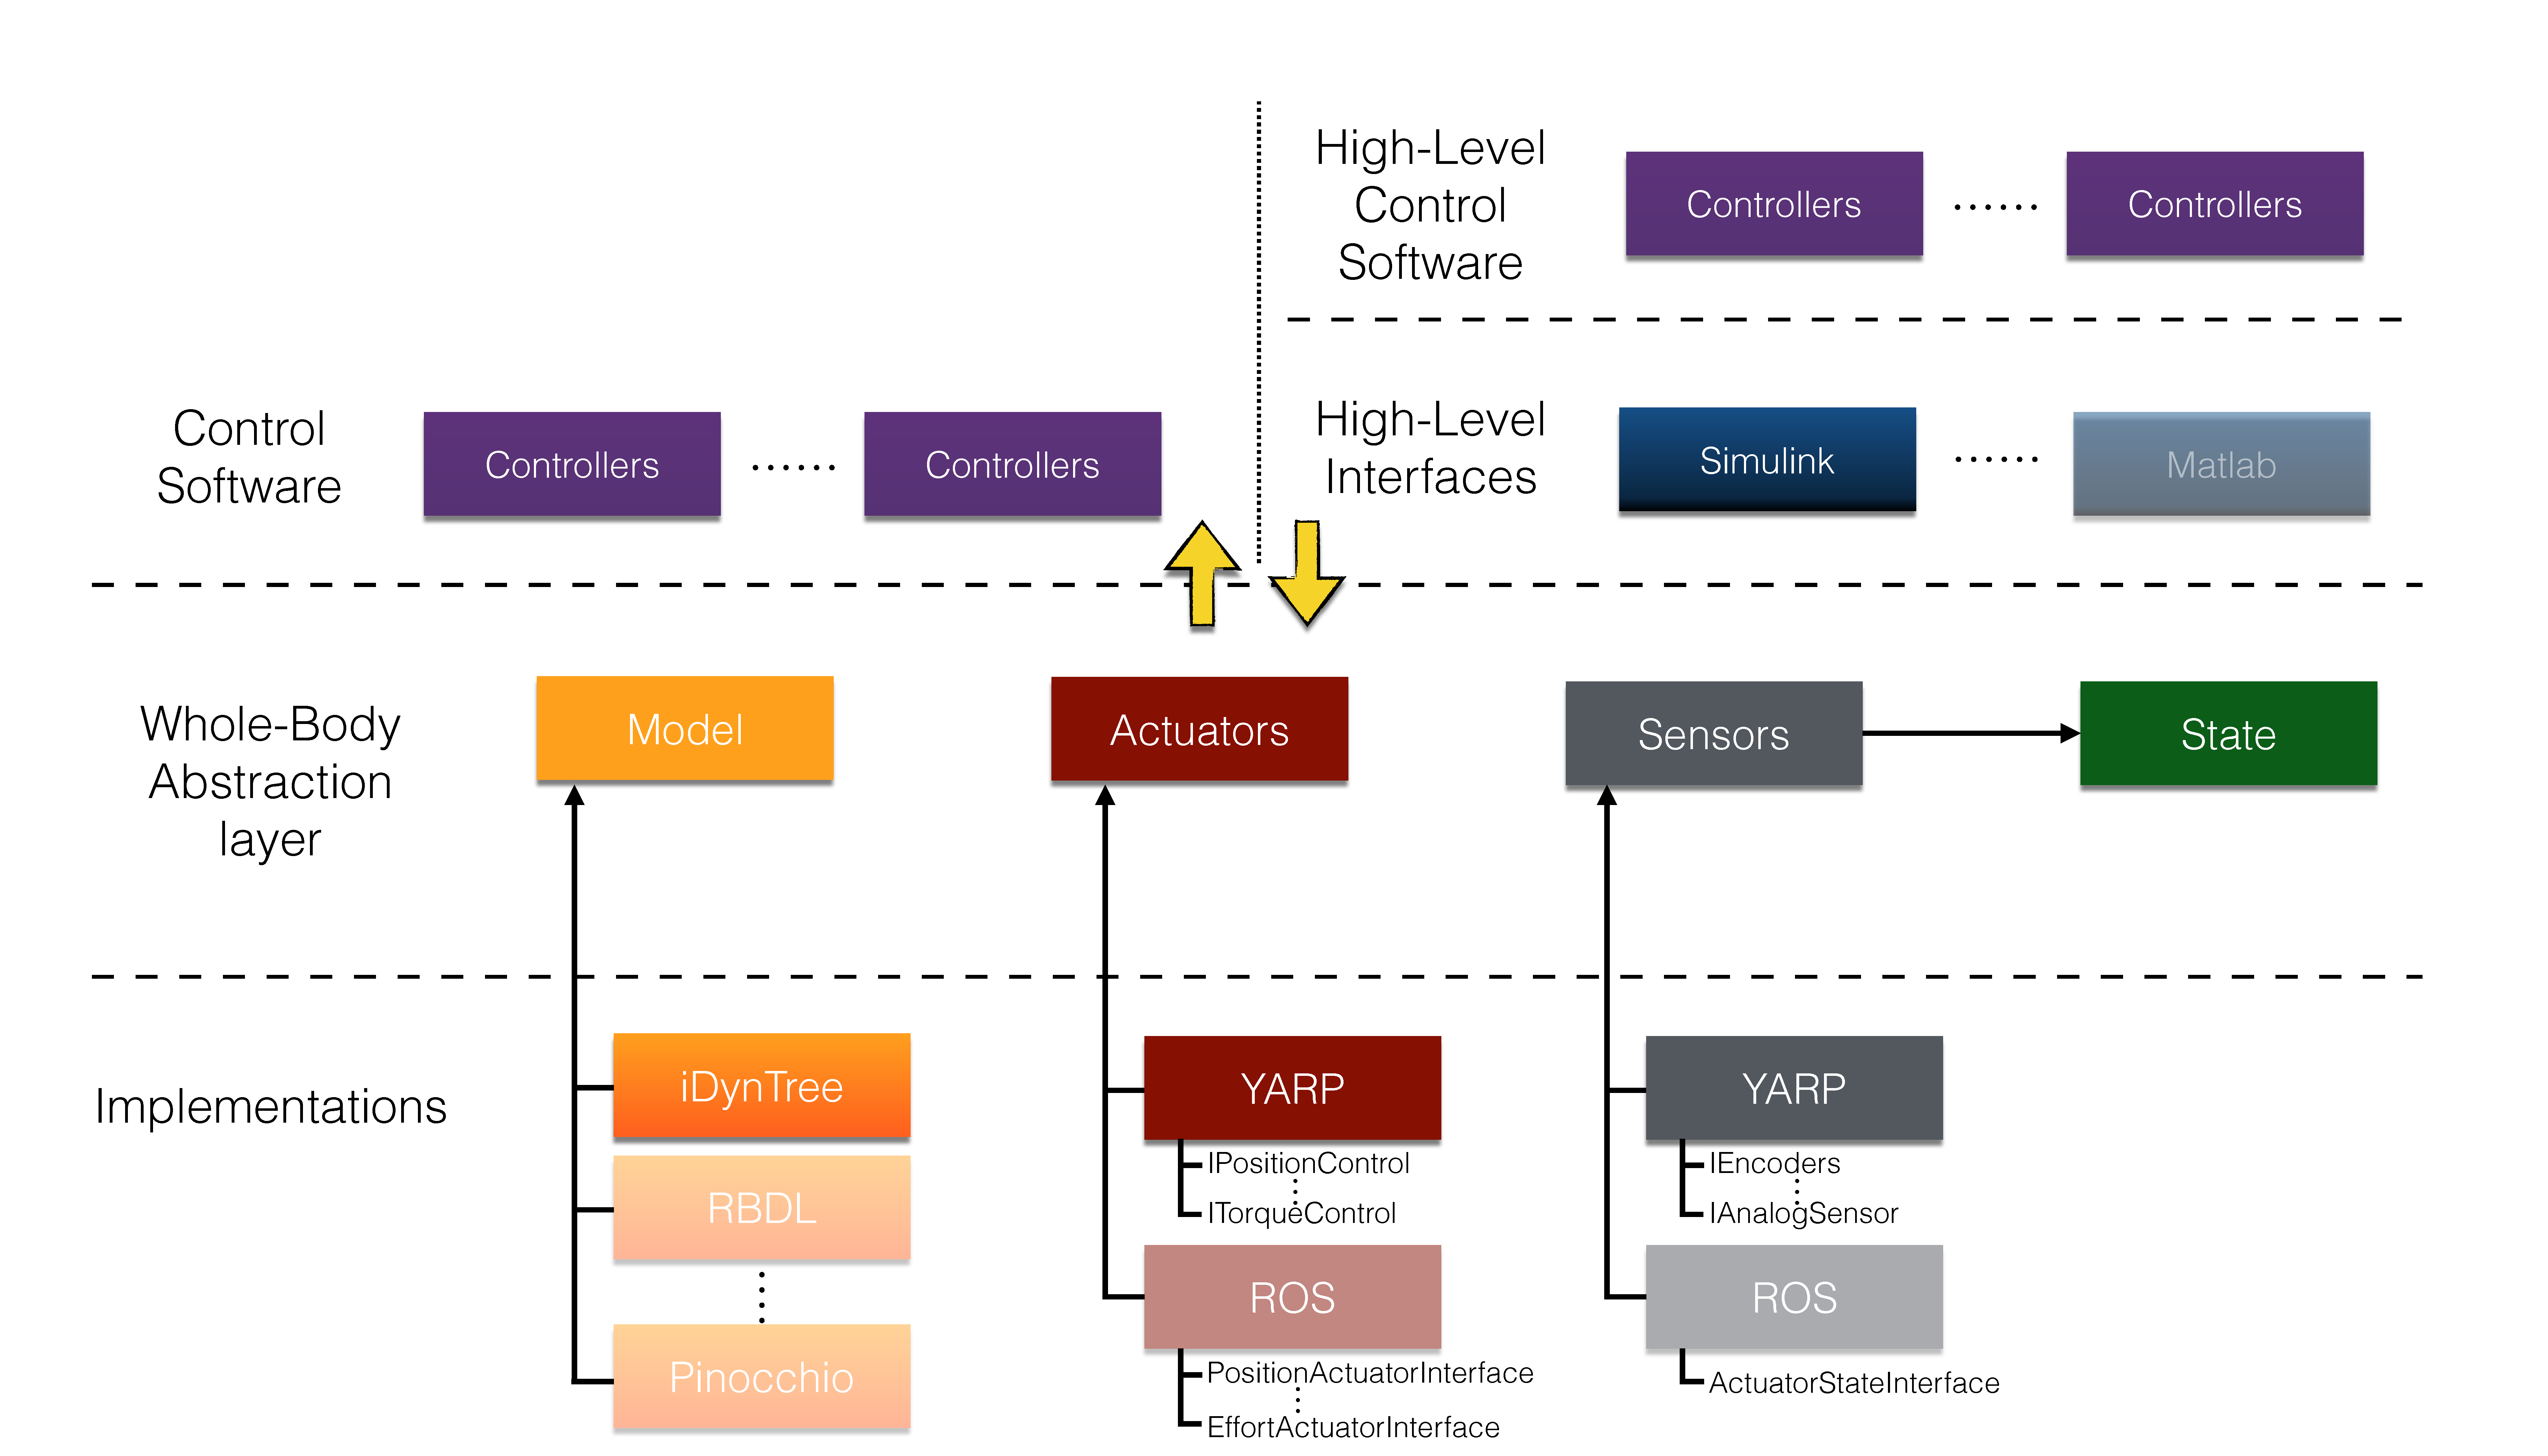
\includegraphics[width=.9\textwidth]{images/WBI_diagram.pdf}
  \caption{Whole-body Interface software architecture}
  \label{fig:images_WBI_diagram}
\end{figure}
%

%% \paragraph{Related Publications:}
%% \begin{itemize}
%%     \item \bibentry{romano2017whole}
%% \end{itemize}


\subparagraph*{System dynamics estimation software. Extension to
environmental compliance estimation (T1.4)}

The goal of T1.4 was to include compliant contact estimation to the software.
This is part of \texttt{codyco-superbuild} software which its details are
reported in deliverables D1.1, D1.2 and D1.3.


\subparagraph*{Extension and enhancement of the iDyn library. (T1.5)}

As part of this task, INRIA developed several software modules which are all
available on github.  These modules which have been used as a support for the
research in the other WPs are:
\begin{itemize}
  \item software and GUI for visualizing the whole-body torques of iCub:
    \url{https://github.com/inria-larsen/icub-wholebody-visualization}
  \item software for interfacing the Geomagic software with Gazebo and use it
    for haptic interaction with iCub:
    \url{https://github.com/inria-larsen/geomagic_touch}
  \item software for learning prioritized controllers, in Matlab, with
    implementation of constrained stochastic optimization algorithms:
    \url{https://github.com/serena-ivaldi/learnOptimWBC}
  \item software for learning Probabilistic Movements Primitives from
    trajectories acquired by demonstrations on iCub:
    \url{https://github.com/inria-larsen/icubLearningTrajectories}
\end{itemize}


During the fourth year, IIT extended the iDynTree library, i.e. the new
version of the iDyn library, to support a new probabilistic based estimation
algorithm with redundant measurements, called Bayesian Estimation for Robot
Dynamics, (BERDY).  BERDY algorithm can be used to estimate the dynamics of
any mechanical system by adopting a sensor fusion approach.  Indeed,
information coming from multiple sensors such as IMUs, force/torque sensors,
etc, can be integrated together with their corresponding variance so as to
obtain the probability density function of the estimate of the whole-body
dynamics of the considered system.  When the Gaussian hypothesis is used, the
dynamics estimation can be obtained by solving a linear system of equations,
which are intrinsically sparse.  This led to the implementation in iDynTree of
a compressed row storage (CRS) scheme for sparse matrices.  Preliminary
results seems to report an increment in the computational performance of about
$40\%$with respect to the dense implementation.  To ease the development of
algorithms and batch data processing, the iDynTree library has been extended
to provide support to Matlab scripting.  It is now possible to call iDynTree
functions directly from Matlab scripts.
%
\begin{figure}[h]
  \centering
    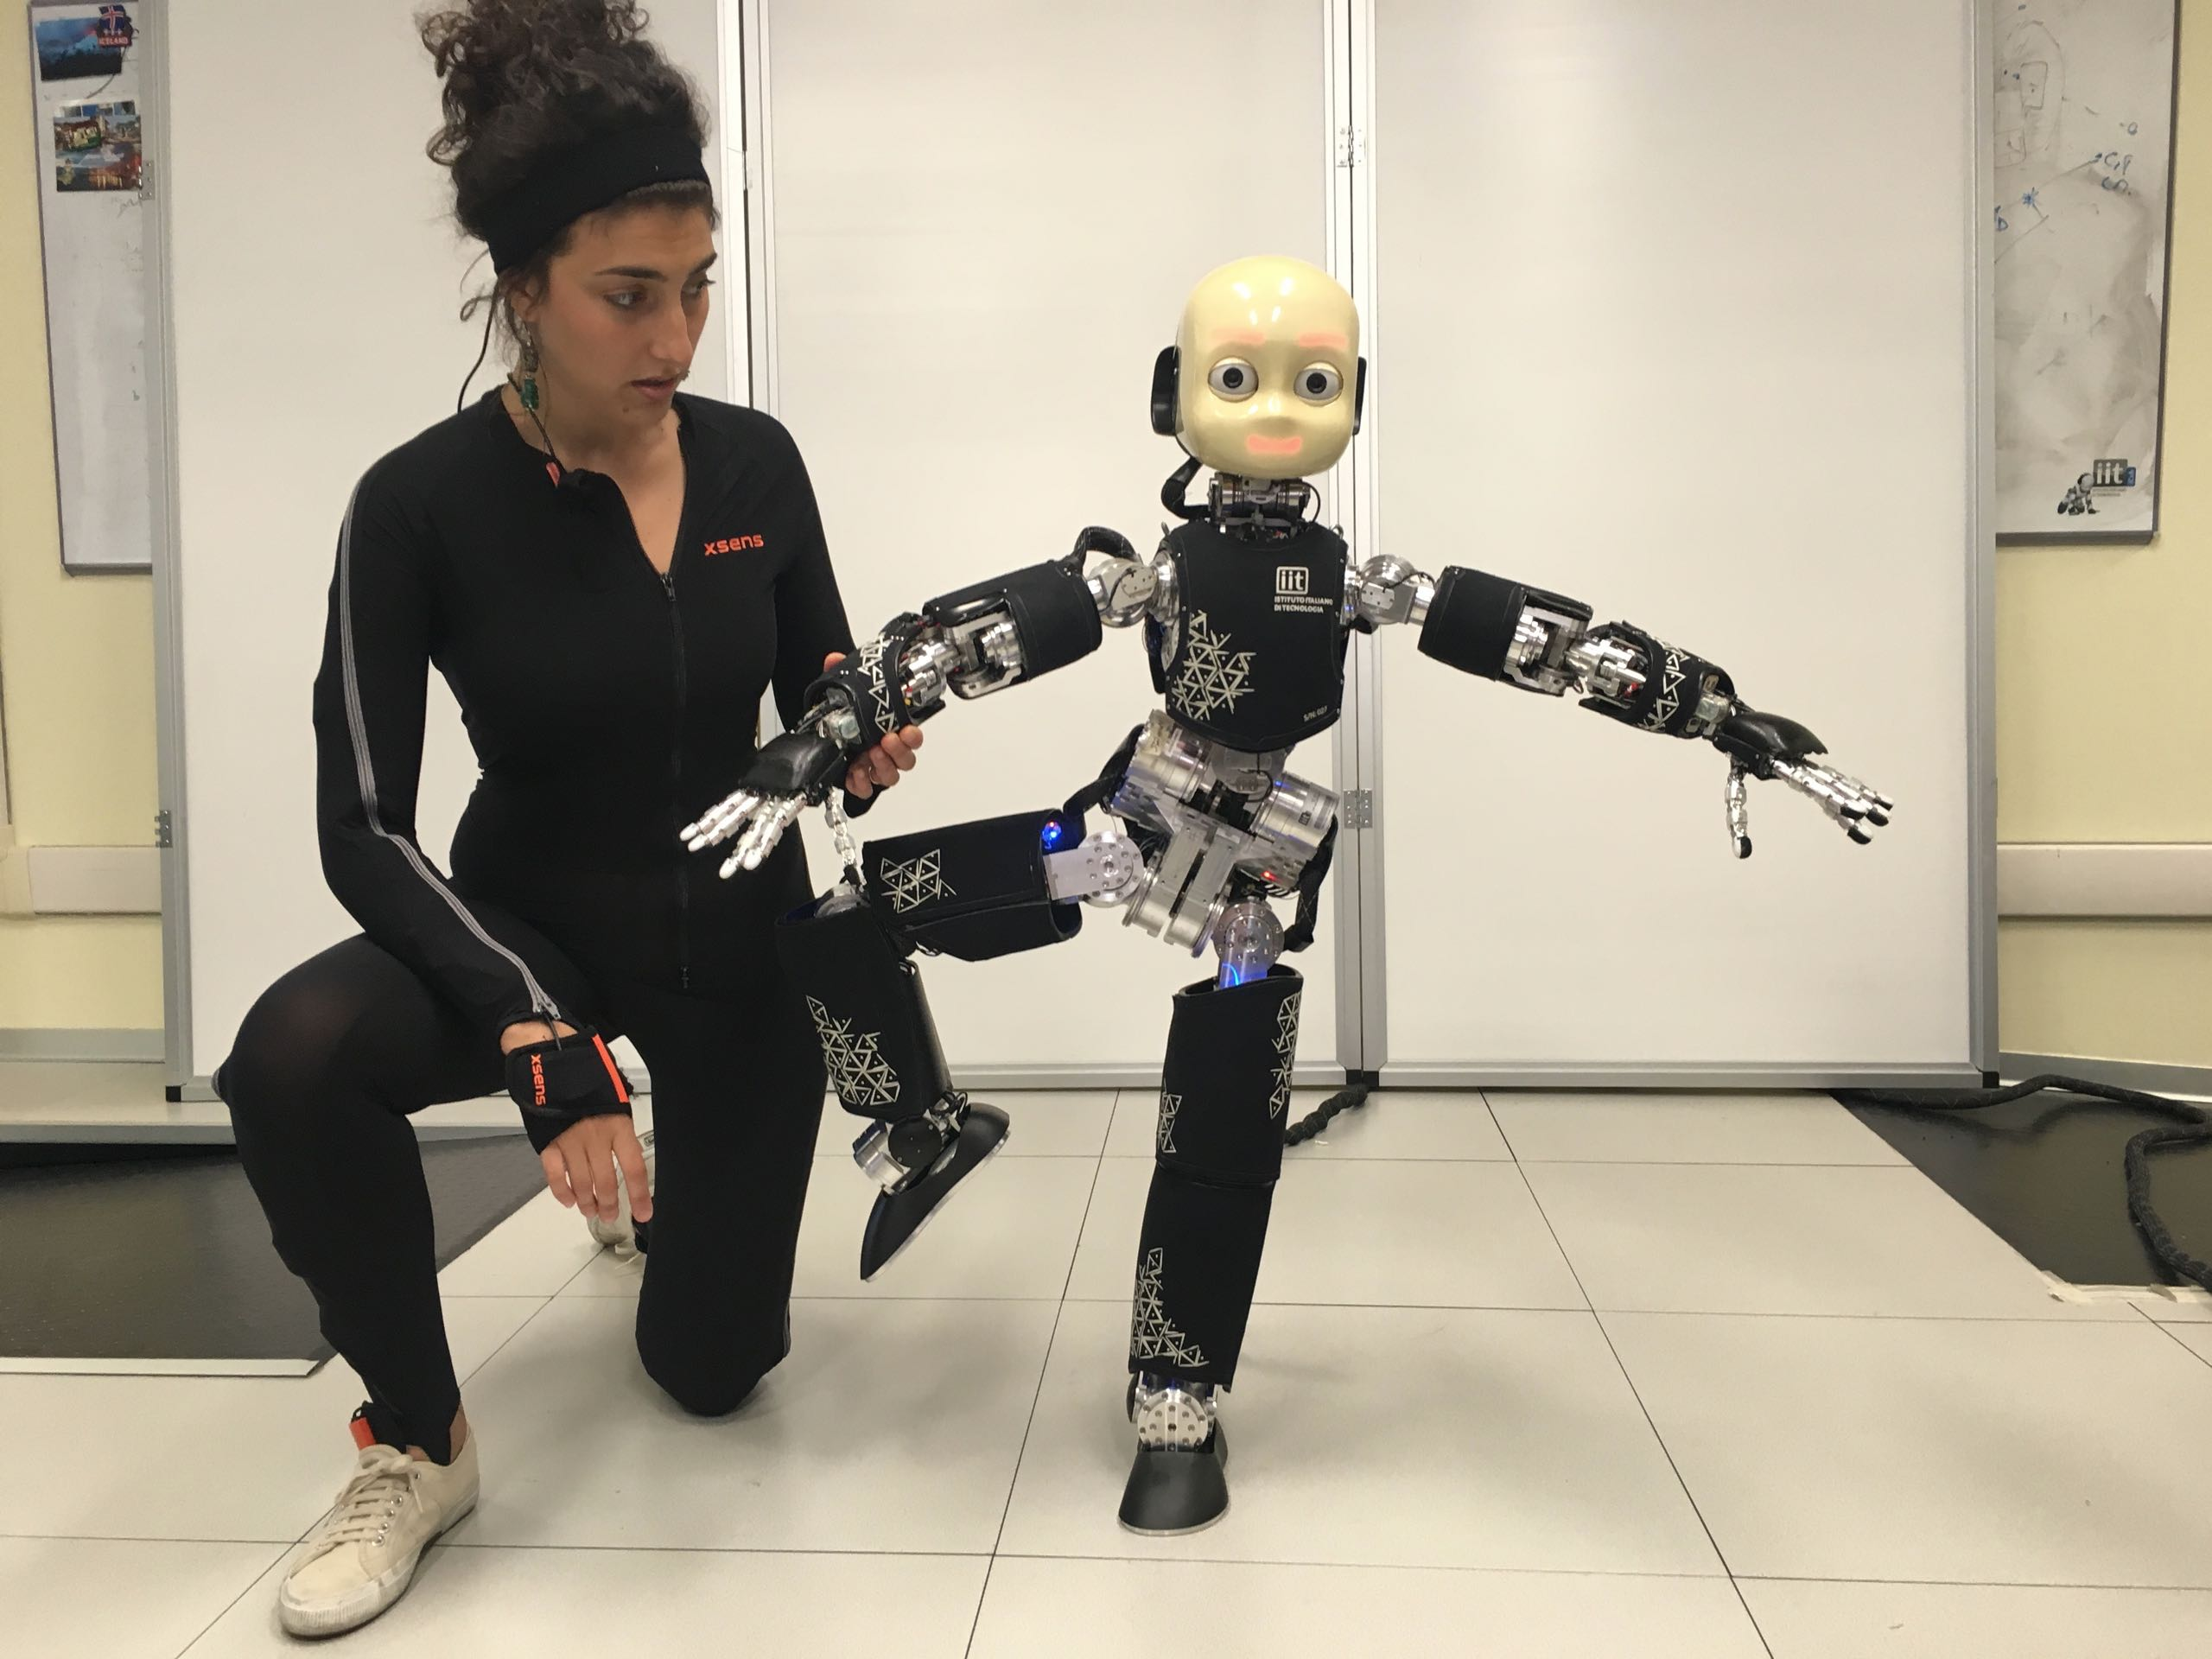
\includegraphics[width=.9\textwidth]{images/suit.jpg}
  \caption{Human interacting with the iCub Robot. The BERDY algorithm can be used to estimate online both the dynamics of the robot and of a human.}
  \label{fig:images_suit}
\end{figure}
%

%% \paragraph{Related Publications:}
%% \begin{itemize}
%%     \item \bibentry{latella2016whole}
%%     \item \bibentry{nori2015simultaneous}
%% \end{itemize}

